% THIS IS SIGPROC-SP.TEX - VERSION 3.1
% WORKS WITH V3.2SP OF ACM_PROC_ARTICLE-SP.CLS
% APRIL 2009
%
% Questions regarding SIGS should be sent to
% Adrienne Griscti ---> griscti@acm.org
%
% Questions/suggestions regarding the guidelines, .tex and .cls files, etc. to
% Gerald Murray ---> murray@hq.acm.org
%
% For tracking purposes - this is V3.1SP - APRIL 2009
%
% Copied from https://github.com/heathermiller/papers-documents/tree/master/rem2013

\documentclass{support/acm_proc_article-sp}
\usepackage{listings}
\usepackage{url}
\usepackage{support/bcprules}
\usepackage{support/prooftree}
\usepackage{support/math}
\usepackage{multicol}
\usepackage{caption}
\usepackage{subcaption}
\usepackage[normalem]{ulem}
\usepackage{color}
\usepackage{graphicx}
\usepackage{hyperref}

\renewcommand{\thesubsection}{\thesection.\alph{subsection}}

\definecolor{blue}{rgb}{0,0,0.5}
\definecolor{red}{rgb}{0.6,0,0}
\definecolor{green}{rgb}{0,0.5,0}
\definecolor{grey}{rgb}{0.2,0.2,0.2}

\lstdefinelanguage{Python}{
keywords={typeof, null, catch, switch, in, int, str, float, self, from, import},
keywordstyle=\color{blue}\bfseries,
ndkeywords={boolean, throw, import},
ndkeywords={return, class, if ,elif, endif, while, do, else, True, False , catch, def},
ndkeywordstyle=\color{blue}\bfseries,
identifierstyle=\color{grey},
sensitive=false,
comment=[l]{\#},
morecomment=[s]{/*}{*/},
commentstyle=\color{green}\ttfamily,
stringstyle=\color{green}\ttfamily,
}

\lstset{language=Python}

\clubpenalty = 10000
\widowpenalty = 10000
\displaywidowpenalty = 10000

% Remove copyright space
\makeatletter
\def\@copyrightspace{\relax}
\makeatother

% comments and notes
\newcommand{\comment}[1]{}
\newcommand{\note}[1]{{\bf $\clubsuit$ #1 $\spadesuit$}}
\newcommand{\ifreport}[1]{#1}
%\newcommand{\ifreport}[1]{}

\newcommand{\todo}{{\bf \colorbox{red}{\color{white}TODO:}}}
\newcommand{\ie}{{\em i.e.,~}}
\newcommand{\eg}{{\em e.g.,~}}
\newcommand{\term}[1]{\mbox{\texttt{#1}}}
\newcommand{\itl}[1]{\mbox{\textit{#1}}}

% commas and semicolons
\newcommand{\comma}{,\,}
\newcommand{\commadots}{\comma \ldots \comma}
\newcommand{\semi}{;\mbox{;};}
\newcommand{\semidots}{\semi \ldots \semi}

% spacing
\newcommand{\gap}{\quad\quad}
\newcommand{\biggap}{\quad\quad\quad}
\newcommand{\nextline}{\\ \\}
\newcommand{\htabwidth}{0.5cm}
\newcommand{\tabwidth}{1cm}
\newcommand{\htab}{\hspace{\htabwidth}}
\newcommand{\tab}{\hspace{\tabwidth}}
\newcommand{\linesep}{\ \hrulefill \ \smallskip}

\newcommand{\sectionline}{%
\nointerlineskip \vspace{\baselineskip}%
\hspace{\fill}\rule{0.5\linewidth}{.7pt}\hspace{\fill}%
\par\nointerlineskip \vspace{\baselineskip}
}

% figures
\newcommand{\figurebox}[1]
{\fbox{\begin{minipage}{\textwidth}
           #1 \medskip
\end{minipage}}}
\newcommand{\twofig}[3]
{\begin{figure*}[t]
     #3\ \hrulefill\
        \caption{\label{#1}#2}
\end{figure*}}
\newcommand{\boxfig}[3]
{\begin{figure*}
     \figurebox{#3\caption{\label{#1}#2}}
\end{figure*}}
\newcommand{\figref}[1]
{Figure~\ref{#1}}

% arrays
\newcommand{\ba}{\begin{array}}
\newcommand{\ea}{\end{array}}
\newcommand{\bda}{\[\ba}
\newcommand{\eda}{\ea\]}
\newcommand{\ei}{\end{array}}
\newcommand{\bcases}{\left\{\begin{array}{ll}}
\newcommand{\ecases}{\end{array}\right.}

\pagenumbering{arabic}
\begin{document}

    \title{Data Mining and Matrices (FSS18) \\ Assignment 3: Non-Negative Matrix Factorization}

    \numberofauthors{1}
    \author{
    \alignauthor
    Steffen Schmitz\\
    \affaddr{University of Mannheim}\\
    \affaddr{stefschm@mail.uni-mannheim.de}
    }

    \maketitle

    %%%%%%%%%%%%%%%%%%%%%%%%%%%%%%%%%%%%%%%%%%%%%%%%%%%%
    %%
    %% 1) Topic Modelling with NMF
    %%
    %%%%%%%%%%%%%%%%%%%%%%%%%%%%%%%%%%%%%%%%%%%%%%%%%%%%

    \section{Topic Modelling with NMF}

    We will first apply NMF to the normalized newsgroup data to discover latent topics.
    Start by computing the NMF optimizing the KL divergence for $r = 4$ factors.
    The output of this step will be two unnormalized matrices $\mathbf{\tilde{L}}$ and $\mathbf{\tilde{R}}$.

    %%%%%%%%%%%%%%%%%%%%%%%%%%%%%%%%%%%%%%%%%%%%%%%%%%%%
    %%
    %% 1.a) Evaluation of NMF results
    %%
    %%%%%%%%%%%%%%%%%%%%%%%%%%%%%%%%%%%%%%%%%%%%%%%%%%%%

    \subsection{Evaluation of NMF results}
    \label{subsec:nmf-r4-evaluation}

    \textbf{Task.} Study the top-10 terms in the right-hand factor matrix $\mathbf{\tilde{R}}$.
    Are the results good?
    To evaluate the results, you must consider the terms associated with each topic and argue why you think they do
    or do not constitute a meaningful topic.

    The rank $r = 4$ non-negative matrix factorization on our document-word matrix produces two matrices
    $\mathbf{\tilde{L}}$ and $\mathbf{\tilde{R}}$.
    According to the lecture slides, we can interpret the matrix $\mathbf{\tilde{R}}$ as a set of parts that are assembled
    with the help of matrix $\mathbf{\tilde{L}}$ to reconstruct our original matrix.

    In our setup the matrix $\mathbf{\tilde{R}}$ has four rows and a column for every word in the original matrix
    $\mathbf{D}$.
    The words with the highest value per row indicate which words are representative for the row and, therefore, for
    the topic that is represented by the row.

    Our original matrix $\mathbf{D}$ includes four topics, Medicine, Space, Christianity and Cryptology, and it is easy
    for us to assign the rows of $\mathbf{\tilde{R}}$ to one of the topics.

    \emph{god}, \emph{christian}, \emph{peopl} and \emph{church} are the four most important words in the fourth row and
    clearly represent the Christianity topic.
    \emph{truth}, \emph{thing} and \emph{homosexu} also appear in the top-10 terms.
    Yet, their relation to the christian religion is not directly obvious, but having in mind that the original matrix
    represents news we can see the religious context.

    This relationship is even more obvious for the other categories. \emph{space}, \emph{launch}, \emph{orbit} and
    \emph{nasa} identify Space, \emph{diseas}, \emph{doctor}, \emph{medic} and \emph{patient} indicate Medicine and
    \emph{encrypt}, \emph{secur}, \emph{govern} and \emph{chip} point to Cryptology.
    We can even deduce the topics without prior knowledge about the topics covered by our initial matrix.

    As before, the allocation of some words is less unambiguous.
    \emph{peopl} is one of the highest rated words in almost all of the categories.
    It is only absent in the topic Space.
    Therefore, it serves as a good example for words that can be used in multiple contexts.
    Hence, it is infeasible to derive the whole topic of a text by looking at only one of the top terms, but a
    combination of frequent words makes guessing the main idea of the text very easy.

    We conclude that the non-negative matrix factorization produces a useful result that reflects the covered topics
    well.

    %%%%%%%%%%%%%%%%%%%%%%%%%%%%%%%%%%%%%%%%%%%%%%%%%%%%
    %%
    %% 1.b) NMF Reconstruction
    %%
    %%%%%%%%%%%%%%%%%%%%%%%%%%%%%%%%%%%%%%%%%%%%%%%%%%%%

    \subsection{NMF Reconstruction}

    \textbf{Task.} Study the reconstructed matrix.
    Does it look like you would have expected?
    Which aspects are covered well?
    Which are not?

    The original matrix is shown in Figure~\ref{fig:1b-original} and the reconstruction in Figure~\ref{fig:1b-reconstruction}.
    For the interpretation we need to keep in mind that the data is sorted by newsgroup.
    This is not exploited by the NMF, but means that rows which are close are likely to respond to similar words.
    \begin{figure}[htbp]
        \centering
        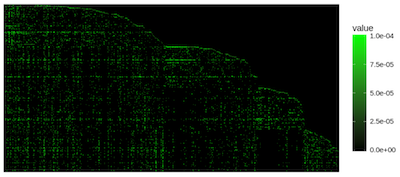
\includegraphics[width=8cm]{images/1b-original.png}
        \caption{Original matrix}
        \label{fig:1b-original}
    \end{figure} \\
    We can see a potential cluster in the top left corner of the original matrix, two in the bottom right and one
    around the middle of the matrix, shifted a little to the top right.
    Keeping in mind that each topic belongs to a quarter of the vertical space, we assume that those clusters contain
    the top-10 words per topic that we analyzed in the previous section.
    \begin{figure}[htbp]
        \centering
        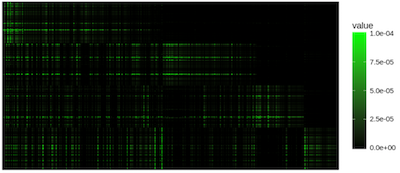
\includegraphics[width=8cm]{images/1b-reconstruction.png}
        \caption{Rank-4 NMF reconstruction}
        \label{fig:1b-reconstruction}
    \end{figure} \\
    The reconstruction retains only the brightest points and lines from the original matrix and amplifies the
    observed structure from the original matrix.
    It is even more obvious where one topic ends and another begins.
    The resulting image seems to consist exclusively of vertical and horizontal lines without the random "noise" points
    that are observed in the original matrix.

    We expected the reconstruction to keep the most important structure of the original matrix, while removing noise.
    This is exactly what we get from it.
    Nevertheless, we are surprised that the outline on the right of the original matrix is not preserved,
    as the step-like decline also seems to contribute to the overall structure.

    Overall, the most prominent clusters are retained, while less bright points and clusters are removed.
    The distinction between the different topics is easier with the reconstructed matrix.

    %%%%%%%%%%%%%%%%%%%%%%%%%%%%%%%%%%%%%%%%%%%%%%%%%%%%
    %%
    %% 1.c) Evaluation of SVD results
    %%
    %%%%%%%%%%%%%%%%%%%%%%%%%%%%%%%%%%%%%%%%%%%%%%%%%%%%

    \subsection{Evaluation of SVD results}

    \textbf{Task.} Take the rank-4 truncated SVD of the data and study the decomposition along the lines mentioned above.
    Compare!

    In the first part of this section we will look at the top-10 largest, absolute values of each row from the right
    singular vectors and in the second part we will evaluate the rank-4 approximation based on the singular value
    decomposition and compare it with the original matrix $\mathbf{D}$.

    The natural interpretation for the right singular values is that if two rows have a similar value in a column of
    $\mathbf{V}$ the attribute is somehow similar.
    If we try to apply this interpretation to our dataset, we see for example that \emph{diet} has a high positive value in
    the second row and a large negative value in the third row.
    We conclude that the second and third row are somehow dissimilar and infer that they represent different topics.
    It would be possible to extend this analysis to multiple columns and increase our confidence that all rows
    are dissimilar from each other, but that would not help our understanding.

    Observing the last row, we see that religious terms score high negative values, while cryptological terms
    score a high positive value.
    In this case the distinction of topics based on the SVD is possible, but all other rows are much harder to interpret.
    This may be the case, because religion is the only non-scientific topic covered in the original matrix and,
    therefore, easier to distinguish.

    All in all, the combination of positive and negative weights makes the interpretation of the SVD less
    intuitive and meaningful.

    Now, we will focus on the rank-4 approximation of our original matrix based on the SVD\@.
    The reconstruction is visualized in Figure~\ref{fig:1c-reconstruction}.
    \begin{figure}[htbp]
        \centering
        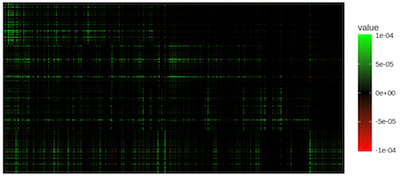
\includegraphics[width=8cm]{images/1c-reconstruction.png}
        \caption{Rank-4 SVD reconstruction}
        \label{fig:1c-reconstruction}
    \end{figure} \\
    In general, the resulting reconstruction looks similar to the rank-4 approximation produced by the rank-4 NMF
    factorization.
    This is expected, because both factorizations try to minimize the difference between the reconstruction and our
    original matrix and, thus, follow the same objective.

    The biggest difference between the two reconstructions is that the SVD reconstruction contains negative values as
    can be infered from the scale next to the chart.
    Examining the matrix closely, we can see a red dot around the middle on the right hand side.
    Although there are no negative values in the original matrix they are included in the reconstructions.
    In this case, unrealistic values help to minimize the difference elsewhere and are therefore included.

    We draw the conclusion that the SVD reconstructs the original matrix very well, but at the cost of uninterpretable
    values.
    The negative values that occur can not be interpreted as a count or percentage and are, therefore, useless.
    The NMF does a much better job at capturing the underlying topics and providing a more intuitive way of interpreting
    the weighting of the attributes.
    It also provides a good reconstruction of the original matrix which is easily interpretable by using the values
    as probabilities for a word to appear in a document.

    Using a NMF for counts or percentages in this case seems superior to the usage of the SVD\@.

    %%%%%%%%%%%%%%%%%%%%%%%%%%%%%%%%%%%%%%%%%%%%%%%%%%%%
    %%
    %% 1.d) Experimenting with the Rank
    %%
    %%%%%%%%%%%%%%%%%%%%%%%%%%%%%%%%%%%%%%%%%%%%%%%%%%%%

    \subsection{Experimenting with the Rank}

    \textbf{Task.} Now try different values of $k$ (at least $r = 2$ and $r = 8$) and repeat the analysis (for NMF only).
    How do the results change?
    Can you name a single best rank?

    We will first compare the top-10 terms produced by the NMF for rank $r \in \{2, 4, 8\}$ and afterwards compare the
    reconstructed matrix of those.

    We already analyzed the top-10 terms in Section~\ref{subsec:nmf-r4-evaluation} and found that the NMF captures
    the covered topics very well and that almost all terms in the top-10 are representative for the whole topic.

    With rank $r = 2$ this distinction between topics based on terms is not that obvious anymore.
    First of all, there are only two topics left - both containing mixed words.
    \emph{god} and \emph{christian} are in the same bucket as \emph{studi} and \emph{effect}.
    Running the NMF multiple times also leads to different weights, which indicates that the optimization gets stuck
    in a local optimum that depends on the initial starting point.
    Overall, the results for $r = 2$ are useless, because we can not draw any conclusions from the resulting topics.

    For rank $r = 8$ we get more useful results than with $r = 2$.
    Every bucket in itself makes sense and can be associated with a topic without difficulties.
    It seems that the topics that are found by NMF are subtopics in the topics that we detected for $r = 4$.
    As an example we may use the two buckets that can be associated with church.
    The eighth bucket contains words like \emph{homosexu}, \emph{sin}, \emph{law} and \emph{christian},
    while the sixth one refers to \emph{bib}, \emph{church}, \emph{cathol} and \emph{truth}.
    To us it looks like the first set of words refers to sins and the law of god, while the second one is a more general
    collection about the church and believing itself.
    We can extend this observation to the other topics like medicine and cryptology.

    Overall, we get useful results for $r = 4$ and $r = 8$.
    Hence, it depends on the context which of those two should be preferred.
    The results for $r = 2$ are too broad and, due to the problem with local optima, unreliable.

    Figure~\ref{fig:1d-rank2-1} and~\ref{fig:1d-rank2-2} show different runs of the rank-2 NMF\@.
    In contrast to the original matrix in Figure~\ref{fig:1b-original}, we see that in each case two of the four
    vertical quartiles look alike.
    \begin{figure}[htbp]
        \centering
        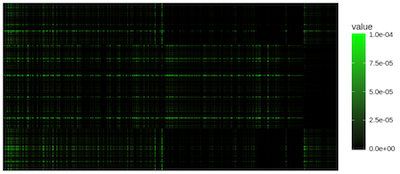
\includegraphics[width=8cm]{images/1d-rank2-1.png}
        \caption{Rank-2 NMF reconstruction 1}
        \label{fig:1d-rank2-1}
    \end{figure} \\
    \begin{figure}[htbp]
        \centering
        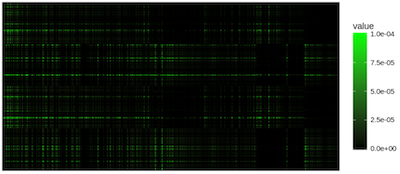
\includegraphics[width=8cm]{images/1d-rank2-2.png}
        \caption{Rank-2 NMF reconstruction 2}
        \label{fig:1d-rank2-2}
    \end{figure} \\
    The basic structure of the original matrix is not retained and, again, the rank-2 NMF produces a bad result.

    We visualize the matrix reconstruction for rank $r = 8$ in Figure~\ref{fig:1d-rank8}.
    \begin{figure}[htbp]
        \centering
        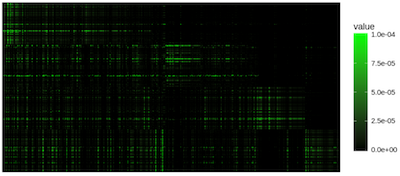
\includegraphics[width=8cm]{images/1d-rank8.png}
        \caption{Rank-8 NMF reconstruction}
        \label{fig:1d-rank8}
    \end{figure} \\
    Compared to the rank-4 approximation from Figure~\ref{fig:1b-reconstruction} the rank-8 approximation
    makes only minor improvements.
    It is hard to identify obvious differences between the two matrices when compared side-by-side.

    In general, we see that the rank-2 NMF produces unreliable results that do not provide much value, because some topics
    are connected, although they are from different categories.
    The rank-8 NMF improves the factorization slightly and can produce useful results if someone wants to split the
    existing topics even further.
    In our opinion, the rank-8 results are to fine-granular.
    Thus, we conclude that the rank-4 NMF produces the best results and recommend to use a rank that is similar
    to the number of topics, if known beforehand.

    %%%%%%%%%%%%%%%%%%%%%%%%%%%%%%%%%%%%%%%%%%%%%%%%%%%%
    %%
    %% 1.e) Gaussian NMF
    %%
    %%%%%%%%%%%%%%%%%%%%%%%%%%%%%%%%%%%%%%%%%%%%%%%%%%%%

    \subsection{Gaussian NMF}

    \textbf{Task.} Apply Gaussian NMF (i.e., using Euclidean norm).
    Do the results change?
    In your opinion, which NMF variant produces better results, if any?
    Argue!

    In this section we will compare the results from the previous sections, which were obtained using the
    Generalized Kullback-Leibler (GKL) as a cost measure for the difference between the original matrix and the factorization,
    with the results obtained by using the Eucledian norm as a cost measure.

    The top-10 terms with their weights seem to be similar to the rank-4 GKL NMF and can be interpreted as in
    Section~\ref{subsec:nmf-r4-evaluation}, but if we look at the weights that are assigned to each word, we can observe
    a difference.
    Interpreting the values as the confidence that a term belongs into this section, we can conclude that the
    Gaussian NMF is more confident in its term allocation than the GKL NMF, although the results are similar.

    We get a similar picture in regard to the reconstruction.
    The resulting matrix is shown in Figure~\ref{fig:1e-gaussian}.
    \begin{figure}[htbp]
        \centering
        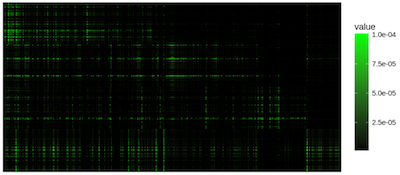
\includegraphics[width=8cm]{images/1e-gaussian.png}
        \caption{Gaussian NMF reconstruction}
        \label{fig:1e-gaussian}
    \end{figure} \\
    The overall structure and the most prominent shapes are similar to the ones in Figure~\ref{fig:1b-reconstruction}.
    Only the values in the Gaussian NMF are slightly lower.
    There are less bright spots and the overall visualization seems more dim.
    Comparing it to the original matrix, the values seem closer together since both are not very bright in most spots.

    Since both cost models try to minimize the distance between the original matrix and the factorization, it is expected
    that the results are close.
    In our opinion it does not make a difference which variant is chosen.

    %%%%%%%%%%%%%%%%%%%%%%%%%%%%%%%%%%%%%%%%%%%%%%%%%%%%
    %%
    %% 2) PLSA
    %%
    %%%%%%%%%%%%%%%%%%%%%%%%%%%%%%%%%%%%%%%%%%%%%%%%%%%%

    \section{PLSA}

    \textbf{Task.} Run NMF with KL divergence and $r = 4$ and factor the resulting decomposition using each of the
    two functions \lstinline{nmf.lsr} and \lstinline{nmf.slr}.
    Study the result.
    Which information is contained in each of the three matrices?
    What can you say about the sum of the entries in each matrix?
    Can you give a probabilistic interpretation of the result (i.e.\@, each entry (i,j) of each matrix)?

    %%%%%%%%%%%%%%%%%%%%%%%%%%%%%%%%%%%%%%%%%%%%%%%%%%%%
    %%
    %% 2.a) nmf.lsr
    %%
    %%%%%%%%%%%%%%%%%%%%%%%%%%%%%%%%%%%%%%%%%%%%%%%%%%%%

    \subsection{nmf.lsr}
    \label{subsec:nmf-lsr}

    \lstinline{nmf.lsr} produces an $m \times r$ matrix $\mathbf{L'}$, an $r \times r$ diagonal matrix $\mathbf{\Sigma'}$,
    and an $r \times n$ matrix $\mathbf{R'}$ such that $\mathbf{\tilde{L}\tilde{R}} = \mathbf{L'}\mathbf{\Sigma'}\mathbf{R'}$,
    and the columns of $\mathbf{L'}$ as well as the rows of $\mathbf{R'}$ sum to one.

    The matrix $\mathbf{\Sigma'}$ is a $4 \times 4$ diagonal matrix that sums to approximately one in our case.
    All values on the main diagonal are approximately $0.25$.
    This corresponds to the fraction that each topic contributes to the number of overall topics.
    Hence, we can interpret $\mathbf{\Sigma'}$ as the frequency of the topic.

    All rows in $\mathbf{R'}$ sum to one and can be interpreted as a probability vector.
    As each row represents one topic and each column a word, we say that the entry $(i,j)$ defines the probability
    that word $j$ appears for topic $i$.
    This indicates that some words are more likely to appear in a topic than others, which matches our presumptions.

    Now we can apply the same logic to the left matrix $\mathbf{L'}$.
    In this case, the columns, representing the topics, sum to one and the rows correspond to documents.
    We can interpret this as the influence that a document has on a topic.
    Documents that have a low value in the left matrix in a column contribute little to the topic, while documents with
    a high value contribute more and have greater influence.

    %%%%%%%%%%%%%%%%%%%%%%%%%%%%%%%%%%%%%%%%%%%%%%%%%%%%
    %%
    %% 2.b) nmf.slr
    %%
    %%%%%%%%%%%%%%%%%%%%%%%%%%%%%%%%%%%%%%%%%%%%%%%%%%%%

    \subsection{nmf.slr}
    \label{subsec:nmf-slr}

    \lstinline{nmf.slr} produces an $m \times m$ diagonal matrix $\mathbf{\Sigma''}$, an $m \times r$ matrix $\mathbf{L''}$,
    and an $r \times n$ matrix $\mathbf{R''}$ such that $\mathbf{\tilde{L}\tilde{R}} = \mathbf{\Sigma''}\mathbf{L''}\mathbf{R''}$,
    and the rows of $\mathbf{L''}$ as well as the rows of $\mathbf{R''}$ sum to one.

    $\mathbf{L''}$ is a $400 \times 4$ matrix and its rows sum to one.
    Again we interpret them as a probability.
    Taking as a example the second row (0.8660983, 0.1332566, 6.426188e-4, 2.530776e-6), we say that document 2
    has a probability of $13\%$ to be in topic 2 and a probability of $87\%$ to be in topic 4.
    All other probabilities are very small and negligible.
    Entry $(i,j)$ in matrix $\mathbf{L''}$ represents the probability that document $i$ is part of topic $j$.

    Matrix  $\mathbf{R''}$ is exactly the same as matrix $\mathbf{R'}$ in Section~\ref{subsec:nmf-lsr}.
    The interpretation is the same.

    Now, only $\mathbf{\Sigma''}$ is left to be interpreted.
    It is a $400 \times 400$ diagonal matrix that sums to one.
    In the previous subsection we interpret the diagonal matrix as the relative frequency of a topic.
    With regards to the documents it makes more sense to take the values in matrix $\mathbf{\Sigma''}$ as relative
    contributions of each document.
    This means that a document with a high value in the diagonal matrix is relevant for the reconstruction, while
    a low value indicates insignificance.

    To verify that those values are truly insignificant, we set all values in the first quartile of $\mathbf{\Sigma''}$
    to 0 and compute the approximated reconstruction.
    Using the Frobenius norm as a measure for the distance between two matrices, we see that both reconstructions are close
    to the original matrix and that the documents with small values in $\mathbf{\Sigma''}$ have little influence.

    %%%%%%%%%%%%%%%%%%%%%%%%%%%%%%%%%%%%%%%%%%%%%%%%%%%%
    %%
    %% 3) Clustering
    %%
    %%%%%%%%%%%%%%%%%%%%%%%%%%%%%%%%%%%%%%%%%%%%%%%%%%%%

    \section{Clustering}

    \textbf{Task.} The documents in the data came from four newsgroups.
    Your task is to cluster the documents in such a way that the clusters correspond to the newsgroups
    (which we can think of as topics).
    To evaluate the quality of the clustering, we treat cluster identifiers as predicted labels and consider the
    accuracy (fraction of correctly predicted labels) and the confusion matrix.
    Cluster the normalized newsgroup data into four clusters using each of the methods below and study the results.
    Also look at the clusters manually.
    Which clustering(s) perform well, which do not?
    Why?

    %%%%%%%%%%%%%%%%%%%%%%%%%%%%%%%%%%%%%%%%%%%%%%%%%%%%
    %%
    %% 3.a) k-Means
    %%
    %%%%%%%%%%%%%%%%%%%%%%%%%%%%%%%%%%%%%%%%%%%%%%%%%%%%

    \subsection{k-Means}
    \label{subsec:k-means}

    Applying $k$-Means to the matrix with $k = 4$ results in a overall accuracy of $26\%$.
    That means that 1 in 4 predictions is correct.
    Looking at the confusion matrix in Figure~\ref{tab:k-means} we can directly see, why this is the case.
    \begin{figure}[htbp]
        \begin{center}
        \begin{tabular}{r | r r r r}
            & 4 & 1 & 2 & 3 \\
            \hline
            4 & 100 & 98 & 99 & 99 \\
            1 & 0 & 2 & 0 & 0 \\
            2 & 0 & 0 & 1 & 0 \\
            3 & 0 & 0 & 0 & 1
        \end{tabular}
        \end{center}
        \caption{k-Means confusion matrix}
        \label{tab:k-means}
    \end{figure} \\
    Almost all documents are in the cluster 4, while all other clusters consists mainly of one or two documents.

    It is likely that this is due to the high dimensionality that is inherent to the data set.
    Although documents may seem close together based on the points the distance between them in the high dimensional
    room is huge.
    This is known as the curse of dimensionality and in particular "\emph{distance concentration}, which denotes
    the tendency of distances between all pairs of points in high-dimensional data to become almost
    equal"~\cite[p.1]{Radovanovic:2010}.

    As all distances are big and nearly equal, the most efficient way for $k$-Means is to put 3 of the 4 centroids onto
    three documents and assigning all other documents to a single centroid, which is, in this case, topic 4.

    %%%%%%%%%%%%%%%%%%%%%%%%%%%%%%%%%%%%%%%%%%%%%%%%%%%%
    %%
    %% 3.b) k-Means on U_4S_4
    %%
    %%%%%%%%%%%%%%%%%%%%%%%%%%%%%%%%%%%%%%%%%%%%%%%%%%%%

    \subsection{k-Means on $\mathbf{U}_4\mathbf{\Sigma}_4$}
    \label{subsec:k-means-svd}

    Using the first two factor matrices of the rank-4 truncated SVD reduces the dimensionality of the input matrix
    from $400 \times 800$ to $400 \times 4$ and shrinks the space substantially.
    This leads to a slightly improved accuracy of $27.75\%$ and the confusion matrix in Figure~\ref{tab:k-means-svd}.
    \begin{figure}[htbp]
        \begin{center}
            \begin{tabular}{r | r r r r}
                & 3 & 4 & 2 & 1 \\
                \hline
                3 & 99 & 89 & 97 & 97 \\
                4 & 0 & 11 & 2 & 3 \\
                2 & 0 & 0 & 1 & 0 \\
                1 & 1 & 0 & 0 & 0
            \end{tabular}
        \end{center}
        \caption{k-Means confusion matrix from rank-4 truncated SVD}
        \label{tab:k-means-svd}
    \end{figure} \\
    Now, there are two cluster centroids which have multiple documents in their cluster, but the overall result is still
    a bad clustering.
    One of the problems may be that all values in the resulting matrix are very small ($\approx$1e-4).
    This means that all distances are approximately the same and the error is small for every possible cluster
    setup.

    %%%%%%%%%%%%%%%%%%%%%%%%%%%%%%%%%%%%%%%%%%%%%%%%%%%%
    %%
    %% 3.c) k-Means on the L̃  matrix of the NMF
    %%
    %%%%%%%%%%%%%%%%%%%%%%%%%%%%%%%%%%%%%%%%%%%%%%%%%%%%

    \subsection{k-Means on the $\mathbf{\tilde{L}}$ matrix of the NMF}
    \label{subsec:k-means-nmf}

    The left matrix $\mathbf{\tilde{L}}$ of the factorization has the same dimensions as our factorization in
    Section~\ref{subsec:k-means-svd}.
    The magnitude of the included values is also similar.
    It likely faces the same issues.

    With an accuracy of $26.75\%$ we again have a minor improvement over the plain $k$-Means model from
    Section~\ref{subsec:k-means}.
    \begin{figure}[htbp]
        \begin{center}
            \begin{tabular}{r | r r r r}
                & 4 & 1 & 2 & 3 \\
                \hline
                4 & 100 & 97 & 97 & 99 \\
                1 & 0 & 3 & 0 & 0 \\
                2 & 0 & 0 & 3 & 0 \\
                3 & 0 & 0 & 0 & 1
            \end{tabular}
        \end{center}
        \caption{k-Means confusion matrix from $\mathbf{\tilde{L}}$ matrix of the NMF}
        \label{tab:k-means-nmf}
    \end{figure} \\
    One major difference that we can infer from the confusion matrix is that there are no mispredictions except for
    cluster 4.
    This indicates that the documents belonging to a topic are closer together than with the previous two models.
    Nevertheless, the issue observed in Section~\ref{subsec:k-means-svd} persists.

    %%%%%%%%%%%%%%%%%%%%%%%%%%%%%%%%%%%%%%%%%%%%%%%%%%%%
    %%
    %% 3.d) k-Means on the L' matrix of factorization L'S'R'
    %%
    %%%%%%%%%%%%%%%%%%%%%%%%%%%%%%%%%%%%%%%%%%%%%%%%%%%%

    \subsection{k-Means on the $\mathbf{{L'}}$ matrix of factorization $\mathbf{L'}\mathbf{\Sigma'}\mathbf{R'}$}

    The result for the $\mathbf{{L'}}$ matrix is similar to the result we obtained from the $\mathbf{\tilde{L}}$
    of the NMF in Section~\ref{subsec:k-means-nmf}.
    We have an accuracy of $26.75\%$ and obtain the confusion matrix shown in Figure~\ref{tab:k-means-lsr}.
    \begin{figure}[htbp]
        \begin{center}
            \begin{tabular}{r | r r r r}
                & 4 & 1 & 2 & 3 \\
                \hline
                4 & 100 & 97 & 97 & 99 \\
                1 & 0 & 3 & 0 & 0 \\
                2 & 0 & 0 & 3 & 0 \\
                3 & 0 & 0 & 0 & 1
            \end{tabular}
        \end{center}
        \caption{k-Means confusion matrix from $\mathbf{{L'}}$ matrix of factorization $\mathbf{L'}\mathbf{\Sigma'}\mathbf{R'}$}
        \label{tab:k-means-lsr}
    \end{figure} \\
    Again, there are no mispredictions, but more documents are falsely assigned to cluster 4.
    We can interpret the confusion matrix similar to the one in Section~\ref{subsec:k-means-nmf}.

    %%%%%%%%%%%%%%%%%%%%%%%%%%%%%%%%%%%%%%%%%%%%%%%%%%%%
    %%
    %% 3.e) k-Means on the L'' matrix of factorization S''L''R''
    %%
    %%%%%%%%%%%%%%%%%%%%%%%%%%%%%%%%%%%%%%%%%%%%%%%%%%%%

    \subsection{k-Means on the $\mathbf{{L''}}$ matrix of factorization $\mathbf{\Sigma''}\mathbf{L''}\mathbf{R''}$}

    Compared to all previous matrices the matrix $\mathbf{{L''}}$ has the additional property that the rows sum to
    one and represent the probability that a document belongs to a specific class.
    In Section~\ref{subsec:nmf-slr} we saw for the second row and for multiple other rows that the NMF is very confident
    in its assignment which means that one document usually gets a value close to one, while all others are approximately
    zero.
    Following this line of argument we would expect the classification to be much better, because we are now able to
    distinguish the documents much better.

    This expectation is confirmed by an accuracy of $95.5\%$ and the confusion matrix in Figure~\ref{tab:k-means-slr}.
    \begin{figure}[htbp]
        \begin{center}
            \begin{tabular}{r | r r r r}
                & 1 & 4 & 3 & 2 \\
                \hline
                1 & 95 & 0 & 1 & 0 \\
                4 & 2 & 98 & 0 & 2 \\
                3 & 2 & 1 & 98 & 7 \\
                2 & 1 & 1 & 1 & 91
            \end{tabular}
        \end{center}
        \caption{k-Means confusion matrix from $\mathbf{{L''}}$ matrix of factorization $\mathbf{\Sigma''}\mathbf{L''}\mathbf{R''}$}
        \label{tab:k-means-slr}
    \end{figure} \\
    All in all, we conclude that the different representations of the NMF lead to improvements in different aspects.
    The $\mathbf{L'}\mathbf{\Sigma'}\mathbf{R'}$ makes it easy to remove insignificant documents, the
    $\mathbf{\Sigma''}\mathbf{L''}\mathbf{R''}$ factorization allows for an effective clustering of the documents into
    topics and, ultimately, $\mathbf{\tilde{L}\tilde{R}}$ helps us to grasp the underlying topics from the most
    representative terms in a topic.

    %%%%%%%%%%%%%%%%%%%%%%%%%%%%%%%%%%%%%%%%%%%%%%%%%%%%
    %%
    %% BIBLIOGRAPHY
    %%
    %%%%%%%%%%%%%%%%%%%%%%%%%%%%%%%%%%%%%%%%%%%%%%%%%%%%

    \bibliographystyle{abbrv}
    \bibliography{support/bib}

\end{document}
